% !TEX root = ../ThesisManuscript_SJ.tex
%
% 	GENERAL DISCUSSION
%___________________________________________________________________________________
\chapter{General discussion}
\label{Discussion}
\markboth{GENERAL DISCUSSION}{}

\section{Summary}

\subsection{Reaching epidemic elimination through the voluntary adoption of prevention}

We modeled the individual response to an epidemic threat through the resolution of a prevention-versus-treatment dilemma, and studied its impact on epidemic spreading. The individual willingness (respectively, refusal) to adopt preventive methods relies on the perception that the strategy of preventing the infection is more (respectively, less) beneficial than facing the risk of being infected, which could lead to acquiring the disease, and consequently being treated. To model the individual-level risk assessment, we assumed that individuals acknowledge some epidemiological data (e.g., the disease prevalence \cite[]{Jijon2017} and the incidence rate \cite[]{Jijon2021}) provided by, for instance, public health authorities, through communication campaigns. 

We used our approach to address two public health issues. First, we studied voluntary vaccination against treatable childhood infectious diseases in a context where efficient, yet imperfect vaccines are available (cf.~\autoref{Vaccine} and \cite[]{Jijon2017}). The results of the vaccination model were obtained analytically, and provided important insights into the system properties, thus constituing a theoretical guide for the coding choices and the interpretation of the results of the second project that involved numerical implementation. Second, we studied the voluntary use of PrEP to avoid HIV infection, among the population of MSM (cf.~\autoref{PrEP} and \cite[]{Jijon2021}). We accounted for population heterogeneity regarding the risk of infection (namely, due to heterogeneity in sexual behaviors). We considered that the high-risk population drives the epidemic, and thus becomes the target population of PrEP implementation policies (unlike childhood vaccination, which is recommended for the vast majority of newborns and young children). 

Our model's main outcome is the prevention coverage reached voluntarily by individuals, expressed as a function of the dynamical system's parameters. In particular, we obtained the voluntary prevention coverage as a function of prevention effectiveness and the relative cost of prevention versus treatment perceived by individuals. From a general point of view, our results suggest that epidemic elimination through the voluntary adoption of prevention is possible, even for imperfect preventive methods, provided that they are highly effective and that individuals perceive the cost of prevention relative to that of treatment being low. 

However, epidemic elimination may be only temporary : we found that the game-theoretic assumption of an equilibrium resolution of the prevention versus treatment dilemma is not ensured. In other words, there is no long-term individual motivation to adopt prevention once the epidemic is eliminated. Indeed, an important decrease in the number of infections may induce individuals to witness less disease burden (such as disease morbidity, difficulties regarding treatment adoption, disease mortality, etc.) and thus, to perceive less benefits from prevention. Therefore, epidemic elimination may induce a higher cost of prevention perceived by individuals, provoking the system dynamics to return to its endemic status.

%; see~\figref{fig:Discussion_Bifurcation} for a simple visualization of this behavior.
%
%\begin{figure}[H]
%	\centering	
%	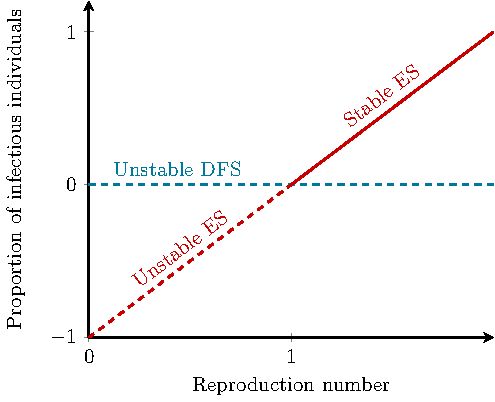
\includegraphics{Figures/Discussion/TikZ_Bifurcation_VolPrev/TranscriticalBifurcation_VolPrev}
%	\caption[ Bifurcation diagram under voluntary prevention]{%
%		{\bf Bifurcation diagram under voluntary prevention}\\
%	A simple diagram to depict how the disease-free equilibrium (DFS) loses its stability when the reproduction number is lower than 1, once the transmission model is coupled to the decision-making model; cf. \figref{fig:Intro_Bifurcation}. The system dynamics tend to go back to the endemic state (ES) and thus, epidemic elimination may be only temporary.}
%	\label{fig:Discussion_Bifurcation}
%\end{figure}

Another key outcome of our model is the effective reproduction number, which we obtained analytically (and not only numerically). This allowed us to study it as a function of the system parameters and thus find the conditions to be met in order to ensure epidemic control (i.e., a decrease in the reproduction number) and/or elimination (i.e., reproduction number below 1). 

In the case of vaccination against childhood infectious diseases, we found that epidemic elimination required the vaccine-induced immunity to be long-lasting, in addition to high vaccine effectiveness. In the case of PrEP uptake against HIV infection, we found that the HIV epidemic may be eliminated by targeting the prevention interventions to those who identify themselves most at risk of infection. We found an expression for the PrEP effectiveness threshold yielding epidemic elimination in terms of the level of risk compensation. In addition, we considered an alternative scenario where individuals misperceive their risk of infection, by acknowledging only the proportion of infected ---and diagnosed--- individuals among their peers. %\rev{and?}

In both projects, we found that risk perception plays a major role in achieving epidemic elimination: the higher the risk perceived, the wider the area where epidemic elimination can be reached --- concerning the perceived cost dimension. That is, if the perceived risk decreases, the cost that individuals are willing to pay to adopt prevention decreases as well, regardless of the level of prevention effectiveness. In other words, if individuals do not perceive themselves as being at a high enough risk of infection, they are less willing to adopt preventive methods. 

\subsection{Establishing public health policies aiming at the end of communicable diseases}

Our results give insights into the issue of voluntary prevention and epidemic behavior in the long run. This allows to place our research within the discussion about sustainability of health behaviors and may thus be helpful for public health policies aiming at epidemic elimination \cite[]{SDG_Goal3}.  

Reaching and maintaining epidemic elimination in the long run requires active efforts to keep the cost of prevention perceived as low, as well as ensuring that individuals have access to accurate, updated epidemiological data allowing them to evaluate their risk of infection. Indeed, global immunization programs aiming to end vaccine-preventable infectious diseases have already pointed to the need of sustaining ``trust in vaccines and immunization services in communities, to increase health literacy with a focus on vaccination at all levels, and to build resilience against misinformation'' \cite[]{WHO_IA2030}; while PrEP programs have identified the need to fight uptake-related difficulties perceived by individuals \cite[]{Desai2018,Sidebottom2018}, misinformation regarding PrEP effectiveness \cite[]{Young2014,Underhill2016} and social stigma and discrimination \cite[]{Young2014,PerezFigueroa2015,Arnold2016}, to increase PrEP adoption and adherence.

Roughly speaking, our results suggest that two main phases should be established by public health policies aiming at disease elimination: i) During an ongoing epidemic, increasing prevention coverage by decreasing the barriers regarding acceptability and accessibility, as well as offering information about the risk of infection and the disease and treatment burden; ii) In the case of epidemic elimination, maintaining high levels of prevention coverage by ensuring accessibility, but also by sharing information about  the achievements of preventive programs and the epidemic severity previous to their implementation. 

In addition, our results may add new perspectives in the discussion about voluntary versus mandatory prevention, by supporting individual informed decision-making, which may actually accompany public efforts towards epidemic elimination, under the proper circumstances.

\section{Limitations}
\subsection{The complexity of modeling human behavior}
As with all modeling studies, ours encounters its limits at representing reality in detail. Simple models are useful to understand epidemic dynamics by interpreting their results, while keeping some flexibility for application to other contexts. However, they may leave aside essential factors reflecting the complexity of human behavior. 

Notably, we use a system of ordinary differential equations to model disease transmission, which may fail to take into account individual heterogeneity. We try to overcome this limitation in the application concerning PrEP and HIV by accounting for two subpopulations, represented by additional compartments. However, we assign fixed parameters for each subpopulation to transit from one compartment to another; that is, all individual behaviors are summarized into an average behavior that is assumed to be the same for all individuals within a given compartment. In addition, we model decision-making as a maximisation of utility, which was mainly based in individuals' perception of the relative cost and the risk of infection. However, individuals may perceive these factors differently and the utility function may also thus be defined to explicitly account for heterogeneity in risk and cost perception. 

In that regard, network-based epidemic models may offer the possibility of modeling population heterogeneity, by defining individuals' profile (demographics, health status, prevention adoption, adherence, etc.) in detail. Network models are also useful to further couple the epidemic spreading and the individual-level decision-making, with information spreading~\cite[]{Chang2020}, which may be interesting to evaluate in a perception-based decision-making framework.


\subsection{Determining and interpreting the relative cost of prevention versus treatment}
Since the decision-making relies not only on monetary, quantitative factors, but also on subjective factors like prevention acceptability and accessibility, as well as self-awareness regarding risk of infection, the resulting values for the total expected utility and the relative cost were read from a qualitative point of view. 
%
Therefore, it is not possible to place a specific situation in a specific point of the {\it cost-axis}: in our framework, one cannot read that a real-life strategy is ``perceived as being $x$ times more beneficial'' than another strategy. 

Nevertheless, the qualitative interpretation of our results might still offer insight about the dynamical system's behavior: from an intuitive point of view, a very low cost perceived by individuals and/or cost reduction may be easier to interpret and to aim to. In addition, our interpretation of the (in)stability of the disease-free equilibria may offer insight on how the dynamical system may respond to interventions. 


\section{Perspectives}

\subsection{Considering other behavioral models}
Also, it could be interesting to account for individuals' acknowledgment of herd immunity to model \textit{free riders}, individuals who decide not to adopt prevention hoping to benefit from others' preventive behaviors. In the case of vaccination, previous studies have found that high vaccination rate decreased the individual's acceptance of vaccination \cite[]{Ibuka2014}. In the case of the use of PrEP, the free-rider phenomenon could be studied by considering, for instance, the probability of undergoing condomless sex with on-PrEP individuals. 

Other modeling choices for the behavioral component may also be interesting for our approach. For instance, including the heterogeneity in the perception of infection risk and cost among individuals, which may help better understanding dynamics in terms of population heterogeneity and developing targeted implementations of prevention programs. Also, considering altruism into the model may allow to study if voluntary prevention coverage may reach levels that optimize the payoff at the collective level \cite[]{Shim2012}. 

%Multi-players games may also be used in order to account for this kind of decision-making.

%\subsection{Relying on other behavioral models}
%\rev{Psychological information-motivation-behavior models ....}

\subsection{Fighting infectious diseases in other socio-economical settings}
Our results point to cost reduction being a key public health's objective to yield epidemic elimination. Our work focuses in fighting epidemic spread within high-income settings, where the notion of cost denotes mostly non-monetary aspects, specially involving the individuals' acceptability of the preventive methods. However, in low-income settings, the consequences of infections may be far more severe, and cost-reducing policies may require to target prevention accessibility rather than prevention acceptability. 

For instance, in the case of the measles epidemiology, the mortality rates can be as high as 2\% to 15\% among children in low-income settings, and mild symptoms like diarrhea and rash can become serious complications, due to malnutrition and hemorrhages \cite[]{Sever2011}. Hence, the MMR vaccine is often well accepted \cite[]{Larson2016}, while a common barrier for vaccination concerns availability issues: as of August 2019, 23 countries had yet to introduce the second dose of MMR vaccine \cite[]{WHO_MeaslesWW2019}. 

Similarly, in the case of the HIV epidemiology, accessing HIV care in low- and middle-income settings and, in particular, the availability of PrEP might still be challenging \cite[]{UNAIDS_Data2019}. Hence, context-specific strategies to facilitate access to PrEP should be implemented \cite[]{Rebe2019}. 


\subsection{Applications to the COVID-19 pandemic}

\noindent From early January 2020 to mid-February 2021, around 109 million cases of SARS-CoV-2\footnote{Severe acute respiratory syndrome coronavirus 2, the causative agent of COVID-19, the severe coronavirus disease. See the review by~\cite{Salzberger2020} for more details on the epidemiology of SARS-CoV-2.} infections resulting in $~\sim2.4$ million deaths were reported to WHO, worldwide \cite[]{WHO_CovidDashboard}. Public health authorities have established a variety of mandatory non-pharmaceutical interventions (NPI) aiming to control de epidemic, including social distancing (i.e., reducing the number of contacts per individual, for instance, by imposing remote work, lockdown, curfews and closing highly-visited places), mask-wearing in public places and promoting regular hands disinfection. NPI have successfully reduced the number of new infections \cite[]{Bo2021}, but strict interventions such as national-level lockdowns and closing schools and stores are not tenable in the long run, so focus was addressed to developing immunization tools. Since mid-December 2020, several two-doses vaccines %preventing COVID-19 as well as preventing SARS-CoV-2 transmission \cite[]{} 
were placed on the market \cite[]{WHO_CovidVaccines}, and vaccination campaigns started around the world. As of mid-February 2021, $\sim180$ million vaccination doses\footnote{These data do not allow to infer the number of vaccinated people, since it is unknown how many of these shots are second doses.} were administered worldwide \cite[]{OWID_CovidVaccination}.

Mathematical models have been used to estimate epidemiological parameters (such as the effective reproduction number and time intervals of disease progression \cite[]{Xiang2021}), as well as to predict the impact of intervention measures \cite[]{Xiang2021} on the still ongoing COVID-19 pandemic. In particular, behavioral epidemiology has been used to study the impact of epidemic control interventions demanding the voluntary participation of individuals, such as social distancing \cite[]{Gupta2020}, stay-at-home (SAH) interventions \cite[]{Kabir2020} and vaccination \cite[]{Choi2020,Jentsch2020}. 
%
All four studies used SEIR-type compartimental model for disease transmission, including symptomatic and asymptomatic individuals. 
%
\cite{Gupta2020} published a working paper where compliance to social distancing interventions was studied via mobility data and in terms of the production and consumption of commodities. They defined the utility function explicitly over regular commodities, occupation and health status. The authors found that information-based interventions had a large impact on mobility during the early stages of the epidemic, and that late adoption of state closure may induce lesser compliance of social-distance adoption and mobility reduction.
%
\cite{Kabir2020} studied the compliance of SAH interventions by including quarantine after exposure to the virus into the transmission model, as well as hospitalizations and immunity after recovery. The payoff depended on the relative costs perceived by individuals and the number of infected individuals. The authors found that individuals' compliance for SAH interventions weans with time. In addition, they studied the final size of the epidemic and the fraction of hospitalized population in terms of the perceived cost and the transmission rate, concluding that SAH and natural immunity complement each other in controlling the epidemic and thus, hospital occupation, as long as cost is perceived low. 
%
\citet{Choi2020} accounted for imperfect vaccination and social distancing (reduction of the number of contacts, by a constant factor) in their transmission model. They analyzed the individuals' expected payoffs (which depended on the strategies' adoption rates and relative perceived costs) when individuals may adopt the strategies of social distancing, vaccination, or both, to avoid infection, finding the threshold relative costs (of vaccination and social distancing) that determined the selection over one strategy over the other. 
%
\cite{Jentsch2020} studied vaccination prioritizing, considering three strategies: i) targeting older first, ii) targeting younger first, iii) vaccinating the whole population uniformly, and iv) a contact-based strategy. The authors used an age-structured compartmental model accounting for imperfect vaccination and contacts by age and location. The decision model concerned the individual adherence to NPI. They calibrated their model using and using mobility data. Their main result in the best strategy (determined by the reduction in the number of deaths), depending on the reported cases and the proportion of vaccinated individuals.

The subject of ending the COVID-19 epidemic at the regional level has been recently discussed. A petition to end SARS-CoV-2 infections at the European level started in Germany in January 2021 \cite[]{ZeroCovid_EU}, suscitating a debate in other European countries, such as France \cite[]{ZeroCovid_FR} and UK \cite[]{ZeroCovid_UK}. Our approach may give  insights into the subject of increasing prevention coverage aiming to COVID-19 elimination, by highlighting how essential an accurate perception of the infection risk and a reduction of the perceived cost of preventing SARS-Cov-2 infection are. 

Individuals' perception on the risk of SARS-CoV-2 infection may be strongly related to the direct experience with the virus at the familiar and professional level \cite[]{Mansilla2020}. In addition, a recent study found that the individuals' knowledge and beliefs about the pandemic were associated with individuals' information sources, which were strongly determined by sociodemographic characteristics \cite[]{Ali2020}. Therefore, availability and broad access to accurate information need to be ensured. Official, governmental sources may help ensuring  individuals' trust in the information, which may translate in the successful adoption of preventive behaviors \cite[]{Lim2020}.

Reducing the perceived cost of prevention in the early stages of an epidemic, specially in a context where therapeutic and immunization tools are not yet available, may be strongly related to disease morbidity and infection scares. However, as times goes by and control measures show their efficacy, individuals' attitudes towards preventive methods may vary more and more. Facilitating the access to both NPI \cite[]{Sugrue2020} and immunization programs \cite[]{Yamey2020} are needed. 

Vaccine attitudes towards vaccination vary widely between countries. A study about the acceptability of the COVID-19 vaccine by \cite{Wuoters2021} found that only 44\% of the French respondents where potentially getting vaccinated, versus a 81\% of the UK responders. Vaccine hesitancy may be addressed, for instance, by increasing communication about vaccines, as well as ensuring broad availability and accessibility \cite[]{Wuoters2021}. In addition, facilitating vaccine adoption may be reached by facilitating the vaccination process itself, for instance, through single-dose vaccines \cite[]{SanchezFelipe2020}.

An additional issue of the COVID-19 epidemic is the high number of asymptomatic infections: an estimated 50\% of infections are produced by asymptomatic cases \cite[]{Johansson2021}. Therefore, testing, tracing and isolating infected individuals has become one of the main strategies to control the epidemic \cite[]{WHO_COVID19Strategy}. Reducing the perceived cost of preventing onward SARS-CoV-2 transmission may thus include facilitating testing. For instance, by establishing mass testing programs or by offering tests through salivar samples instead of nasopharyngeal swabs \cite[]{Yee2021}, as well as at-home alternatives \cite[]{ValentineGraves2020}. 

\subsection{The impact of the COVID-19 pandemic on prevention interventions against measles and HIV}
The completion of our research project took place before the emergence of the COVID-19 pandemic. Ours and future modeling studies will need to take into account the impact of the COVID-19 on other epidemics to ensure accurate model fitting and outcomes from early 2020 on, and during the COVID-19 emergency.

Indeed, the COVID-19 epidemic impacted childhood immunization, with 37 countries delaying immunization activities during the first wave of the epidemic \cite[]{WHO_CovidMeasles}. Hence, to maintain measles on the path of epidemic elimination, public health authorities around the world will need to address the decrease in prevention coverage that the COVID-19 epidemic provoked during the year 2020. 

The COVID-19 epidemic also impacted PrEP uptake in France. The so far increase in PrEP use in France was slower during the first semester of 2020 (cf.~\figref{fig:PrEP_IdF}). A survey made to $\sim8\,350$ French MSM regarding their sexual behaviors during the period June-July 2020 found that 60\% of respondents had declared a complete drop in casual sexual encounters, and that 59\% of PrEP users had stopped using PrEP due to a decrease in sexual activity \cite[]{Velter2020}.

%\textit{Applications to other epidemics}
%
%Our results may offer some particularly helpful insight for the global efforts to end polio, tuberculosis, malaria and other communicable diseases before 2030 \cite[]{SDG_Goal3}, as well as the global immunisation plan \cite[]{WHO_GVAP2018}. On the other hand, considering the prevention versus treatment dilemma and thus including individuals' decision-making into mathematical models may also yield new insights into the impact of voluntary prevention on the epidemic in the context of other infectious diseases that are in the path towards elimination, such as hepatitis B, human papillomavirus \cite[]{Basu2008}, hepatitis C and syphilis.

\section{Conclusion}
In conclusion, the methods developed in this doctoral research program allowed us to study infectious disease epidemics in terms of individual's attitudes towards the available preventive methods against infection, as well as their perception of the risk of infection. In particular, we focused on studying the conditions under which epidemic elimination could be reached through the voluntary participation of the target population.

We found that public health programs may yield epidemic elimination, provided that i) highly-effective preventive methods are available and perceived as being at low cost; and ii) that so individuals have a fair perception of their risk of infection. However, once the epidemic is eliminated, active efforts from public health authorities are needed to maintain the individual perception of the prevention cost low, so the willingness to keep using prevention maintains voluntary-prevention coverage at sufficiently high levels.